\documentclass[12pt]{book}

\title{The dark version\\ \textit{better to burn out than to fade away}
\begin{center}
\includegraphics[width=2in]{org/art/cannabis.png}\end{center}
}

%\usepackage[margin=1in]{geometry}

\usepackage{listings}
\lstset{numbers=left,basicstyle=\scriptsize \ttfamily \color{codecolour},language=}

\usepackage{color}
\definecolor{codecolour}{RGB}{180, 180, 180}
\definecolor{tipcolour}{RGB}{50, 50, 50}
\definecolor{pagecolour}{RGB}{180, 180, 180}
\pagecolor{black}
\color{pagecolour}

\usepackage{graphicx}
\usepackage{wrapfig}

\begin{document}
\maketitle

% Where to find things
% Your best friends (npm and stackoverflow) - could be node mailing list but there's lot of weed and watching people do amazing stuff might be a demotivating for a beginner. Of course, its all about the way you see it. You could have thick skin or really able to appreciate how wonderful people are. The later one being rare.
% npm syntax 

\chapter{Introduction}

\begin{wrapfigure}{r}{2in}
\begin{center}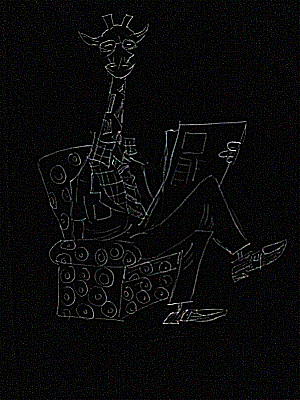
\includegraphics[width=2in]{org/art/takingHelp.png}\end{center}
\end{wrapfigure}

Are you demotivated? Do you find the world uninspirational. Do you find yourself yourself left out in the world without keeping pace with rapidly progressing technology. You may probably find peace in development. Development is awesome because it gives you the feeling of God. You create and see your things working.
\linebreak
\par
As a developer, its your religion to try every stuff out there. This book is about taking shortcuts to get your 'thing' running. This book targets only a specific set of technology. You may choose to differ and take a different path.
\linebreak
\par
Hopefully, it will give you a drift and get started. You will have to solve your itches and tackle issues yourself. However, as a general rule of thumb a search engine, say, Google will be your best friend. And there's no better platform for your programming queries than StackOverflow. Most of your queries will be already answered there. When you feel like expert of nodejs and can't find answers online, you can even join the mailing list.
%You could opt for asking questions at the nodejs mailing list, but subscribing will mean lot of emails every day as node is quite a hot topic these days.
%Also, it might be demotivational because you will see people building fantastic things and their progress is much faster than yours.
%So, initially you might want to focus on fixing your problems before you catch speed.
%the survival tale/keeping alive - airbnb for motivation

%\begin{flushright}\textit{Its better to burn out than to fade away.}\end{flushright}
%What is this book about? This book is intended to serve as a tutorial to build your applications quickly.


\chapter{Quick Launch}
\begin{flushright}\textit{It seems I am on speed.}\end{flushright}

\begin{wrapfigure}{r}{2in}
\begin{center}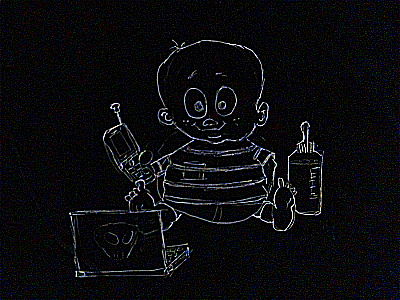
\includegraphics[width=2in]{org/art/getStartedHigh.png}\end{center}
\end{wrapfigure}

Nothing gives a better kick than working and releasing fast. The following code will get you a ``launching soon'' page ready with beta invite albeit manually. It requires node.js, an evented IO framework by Ryan Dahl. The code itself is written in coffeescript, a language by Jeremy Ashkenas.
First be comfortable with code and the fact that this small code will get us started and then we can move on to get it working.

\vspace{0.6cm}\lstinputlisting{app/stage1/server.coffee}\vspace{0.6cm}

%tip
\colorbox{tipcolour}{\tiny \textsc{Tip} \small Use commercial solutions like unbounce to set up quick sign up page}


%\chapter{Working Model}
%\begin{flushright}\textit{If it doesn't work, it doesn't exist.}\end{flushright}

%\begin{wrapfigure}{r}{2in}
%\begin{center}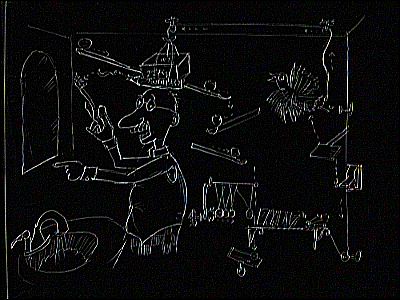
\includegraphics[width=2in]{org/art/workingModel.png}\end{center}
%\end{wrapfigure}

%Last stage was a baby's task. Lets get real and get a working model. To keep it simple, lets stick with simplest authentication via facebook and build upon existing hardwork. MongoDB will be used for storage, though a document based database is not really an ideal choice for the purpose. 


\chapter{Express}
\begin{flushright}\textit{Run. Run. Run.}\end{flushright}

\begin{wrapfigure}{r}{2in}
\begin{center}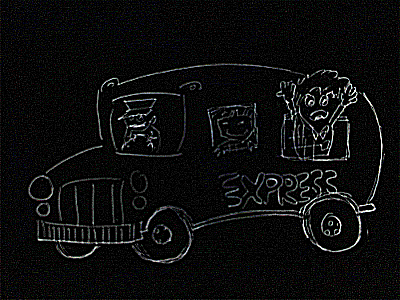
\includegraphics[width=2in]{org/art/fasterEasier.png}\end{center}
\end{wrapfigure}

Time to take the express. A quick reorganization of code so as to switch to a big framework which will make life easier in long run. As you can figure out we don't need to parse req.url and add switch statement to handle different url, if we stuck to last example. Express makes routing a breeze.

\vspace{0.6cm}\lstinputlisting{app/stage2/server.coffee}\vspace{0.6cm}



\chapter{Database}
\begin{flushright}\textit{You can has data.}\end{flushright}

\begin{wrapfigure}{r}{2in}
\begin{center}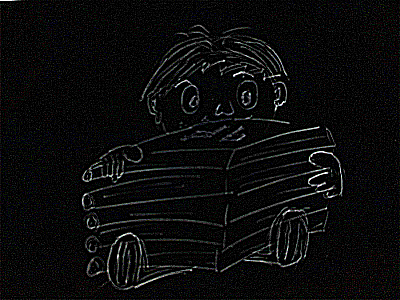
\includegraphics[width=2in]{org/art/dataStorage.png}\end{center}
\end{wrapfigure}

MongoDB will store our data. Note that we have to think asynchronously. The database choice here was dictated more by ease rather than a good fit. In fact, a document based database in not really optimal for storing relational data.
Lets focus on the working example which pulls the data from the database. Visit mongodb website for installation, building a database and storing dummy data. We will use mongoose module to interact with the server.

\vspace{0.6cm}\lstinputlisting{app/stage3/server.coffee}\vspace{0.6cm}

%tip
%\noindent
Movie data can be inserted via mongo command line interface \\
\colorbox{tipcolour}{\tiny \textsc{Tip} \small ./mongodb-linux-i686-1.6.5/bin/mongod --dbpath ./data/db/ } \\
\colorbox{tipcolour}{\tiny \textsc{Tip} \small ./mongodb-linux-i686-1.6.5/bin/mongo localhost/db } \\
\par

%or via node application
%\begin{lstlisting}
%mongoose = require 'mongoose';
%mongoose.connect 'mongodb://localhost/db';
%require './models/movie';
%movie = mongoose.model 'movie';
%d = new movie();
%d.id = 2;
%d.name = 'Andaz Apna Apna';
%d.save (err) ->
%	if (err)
%		console.log 'error: ' + e;
%	mongoose.disconnect();
%\end{lstlisting}




\chapter{Intermission}
\begin{flushright}\textit{Organize your data before you die.}\end{flushright}

\begin{wrapfigure}{r}{2in}
\begin{center}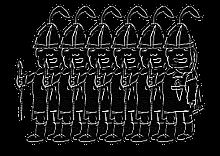
\includegraphics[width=2in]{org/art/organized.png}\end{center}
\end{wrapfigure}

We will stick to a common layout in order to keep the code organized in long run. It also makes it easier to understand and maintain. Here, models directory will contain the data models corresponding to the database. Controllers will be handlers of different type of requests. The views will contain Jade templates which will be rendered by the jade module.
\linebreak

\begin{verbatim}
       app.coffee               (our application)
       |--models                (contains data models)
       |--views                 (jade templates)
       |--controllers           (handler for different requests)
       |--data                  (data storage)
          |--db
       |--public                (static content)
          |--js
          |--css
          |--img
\end{verbatim}

\par
\vspace{1cm}

According to this scheme, the contents will now be\\
\lstinputlisting[title={app.coffee}]{app/stage4/app.coffee}\vspace{0.6cm}
\lstinputlisting[title={movie controller}]{app/stage4/models/movie.coffee}\vspace{0.6cm}
\lstinputlisting[title={homepage controller}]{app/stage4/controllers/home.coffee}\vspace{0.6cm}
\lstinputlisting[title={movie model}]{app/stage4/controllers/movie.coffee}\vspace{0.6cm}

Current example doesn't really use templates because we are just refactoring the code from last chapter. But the organisation reflects how we want to categorize similar type of source files in the same organisation hierarchy under same directory.


%Dealing with image data
%We can store it at EC2 and refer to its location in the database

\end{document}
